\documentclass[10pt,a4paper]{article}

\usepackage[a4paper,margin=0.55in]{geometry}
\usepackage{titlesec}
\usepackage{enumitem}
\usepackage{xcolor}
\usepackage{tabularx}
\usepackage{graphicx}
\usepackage{array}
\usepackage[normalem]{ulem}
\usepackage[
    colorlinks=true,
    urlcolor=blue,
    linkcolor=black
]{hyperref}

\setlist[itemize]{
    leftmargin=1.2em,
    itemsep=1pt,
    topsep=2pt,
    parsep=0pt,
    partopsep=0pt
}

\pagestyle{empty}

\titleformat{\section}
{\large\bfseries}
{}
{0em}
{}[\titlerule]

\titlespacing*{\section}
{0pt}{6pt}{4pt}

\begin{document}

\begin{center}
\begin{tabularx}{\textwidth}{X r}

% Left Side
\begin{minipage}{0.65\textwidth}
\begin{minipage}{0.22\textwidth}
    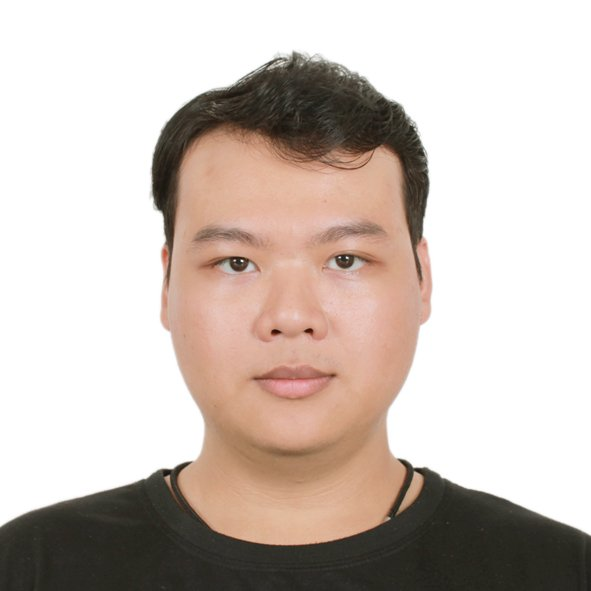
\includegraphics[width=3cm,height=3cm]{assets/Avatar.jpg}
\end{minipage}
\hfill
\begin{minipage}{0.72\textwidth}
    {\LARGE \textbf{Nguyen Tuan Khoa}}\\[6pt]
    \textbf{Software Developer}
\end{minipage}
\end{minipage}

&

% Right Side
\begin{minipage}{0.3\textwidth}
\raggedleft
\footnotesize

Vuon Lai Ward, Ho Chi Minh City\\[2pt]

(+84) 909 801 582\\[2pt]

\href{mailto:khoanguyen030803@gmail.com}
{khoanguyen030803@gmail.com}\\[2pt]

\href{https://github.com/AlexPerdron}
{github.com/AlexPerdron}

\end{minipage}

\end{tabularx}
\end{center}

\section*{Objectives}

As a final-year IT student with hands-on experience in Back-End, Front-End, and Mobile development, I am eager to expand my technical expertise by taking on new challenges and opportunities that enhance my skills and industry knowledge.

\section*{Education \& Experience}

\textbf{International University -- Vietnam National University HCMC}
\hfill \textit{2021 -- Present}

\vspace{0.2cm}

\textit{Bachelor of Computer Science}

\begin{itemize}[leftmargin=*]
    \item Coursework: Software Architecture, UI Design and Evaluation, Scalable and Distributed Computing, Principles of Database Management.
\end{itemize}

\vspace{0.2cm}

\noindent
\textbf{Backend Intern -- Anh Quan Technology Company}
\hfill \textit{Feb 2024 -- May 2024}

\begin{itemize}[leftmargin=*]
    \item Developed and maintained the company website and APIs.
    \item Researched new technologies and frameworks for company projects.
\end{itemize}

\vspace{0.2cm}

\noindent
\textbf{Software Engineer Intern -- VNEMEX Company Limited}
\hfill \textit{Jan 2025 -- July 2025}

\begin{itemize}[leftmargin=*]
    \item Developed UI for both website and mobile interfaces.
\end{itemize}

%====================
% Technologies
%====================

\section*{Technologies}

\begin{itemize}[leftmargin=*]
    \item \textbf{Languages:} HTML/CSS, C/C++, JavaScript, TypeScript, SQL.
    
    \item \textbf{Technologies:} React.js, Node.js, Express.js, React Native, RESTful API, GraphQL, Postgraphile, Microsoft SQL Server, MongoDB, Docker, Supabase.
    
    \item \textbf{Other:} Git, Tailwind CSS, Figma.
\end{itemize}

%====================
% Projects
%====================

\section*{Projects}

\noindent
\textbf{Bomberman Adventure}
  \hfill
\href{https://github.com/AlexPerdron/Bomberman-Adventure}
{\uline{github.com/AlexPerdron/Bomberman-Adventure}}

\begin{itemize}[leftmargin=*]
    \item Developed a classic Bomberman game with a team of five to deepen understanding of object-oriented programming.
    \item Programming language used: Java.
\end{itemize}

\vspace{0.2cm}

\noindent
\textbf{Catch Me If You Can}
\hfill
\href{https://github.com/AlexPerdron/Catch-Me-If-You-Can}
{\uline{github.com/AlexPerdron/Catch-Me-If-You-Can}}

\begin{itemize}[leftmargin=*]
    \item Applied data analysis and path-finding algorithms in a game-based project.
    \item Programming language used: Java.
\end{itemize}

\vspace{0.2cm}

\noindent
\textbf{TASKing}
\hfill
\href{https://github.com/AlexPerdron/task_manager_be}
{\uline{github.com/AlexPerdron/task\_manager\_be}}

\begin{itemize}[leftmargin=*]
    \item Developed a web-based application for managing team and personal tasks.
    \item Developed APIs and used Docker and Render for deployment.
    \item Tools used: TypeScript, MongoDB, Prisma, Node.js, Express.js, Docker, RESTful API, Render.
\end{itemize}

\vspace{0.2cm}

\noindent
\textbf{Family Tree Management System}
\hfill
\href{https://family-tree-frontend-adfa.onrender.com/}
{\uline{Demo Link}}

\begin{itemize}[leftmargin=*]
    \item Designed and developed a full-stack web-based application for managing and visualizing family trees.
    
    \item Supported both Lunar and Gregorian calendars for genealogical events and anniversaries.
    
    \item Implemented public family tree sharing with secure access control for external viewers.
    
    \item Tools used: TypeScript/JavaScript, React, Next.js, Tailwind CSS, Node.js, Express.js, PostgreSQL, Supabase, RESTful API, Render.
\end{itemize}

\vspace{0.2cm}

\noindent
\textbf{Parcel Locker} \hfill \textit{2024}

\begin{itemize}[leftmargin=*]
    \item Developed a mobile application for managing customer packages in a locker system.
    
    \item Managed UI teams and coordinated collaboration between design and development.
    
    \item Tools used: React Native, Tailwind CSS, Figma.
\end{itemize}

%====================
% Certifications
%====================

\section*{Certifications}

IELTS 6.5 (2022)

\end{document}